\chapter{A természet, mint eszköz és forrása}

Az emberek vizuális lények ezért a minket körülvevő tárgyak formája mintázata (\ref{fig:nat_pet}. ábra) befolyásolja a mentális és lelki állapotunkat is. Ezeknek az organikus mintázatoknak a hatása közismert és jól dokumentált, mint ahogy az \cite{jo2019physiological} -ben is olvasható. Ezek az organikus mintázatok lehetővé teszik, hogy az ember fenntartsa azt az ősi kapcsolatot, ami össze köti a természettel. 

\begin{figure*}[ht!]
	\centering
	\begin{subfigure}[b]{0.225\textwidth}
		\centering
		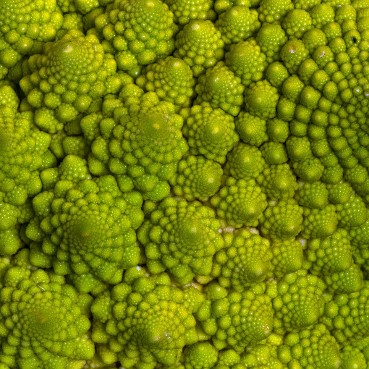
\includegraphics[width=\textwidth]{img/nat_pat_01.jpg}
		\caption{}    
	\end{subfigure}
	\hspace{10 mm}
	\begin{subfigure}[b]{0.225\textwidth}  
		\centering 
		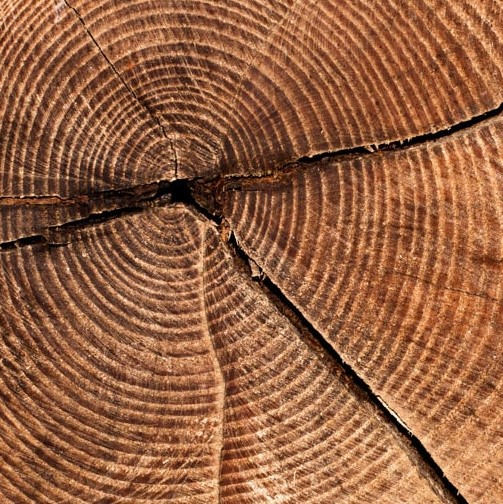
\includegraphics[width=\textwidth]{img/nat_pat_02.jpg}
		\caption{}  
	\end{subfigure}
	\vskip\baselineskip
	\begin{subfigure}[b]{0.225\textwidth}   
		\centering 
		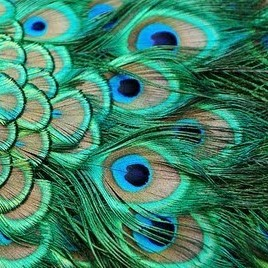
\includegraphics[width=\textwidth]{img/nat_pat_03.jpg}
		\caption{}    
	\end{subfigure}
	\hspace{10 mm}
	\begin{subfigure}[b]{0.225\textwidth}   
		\centering 
		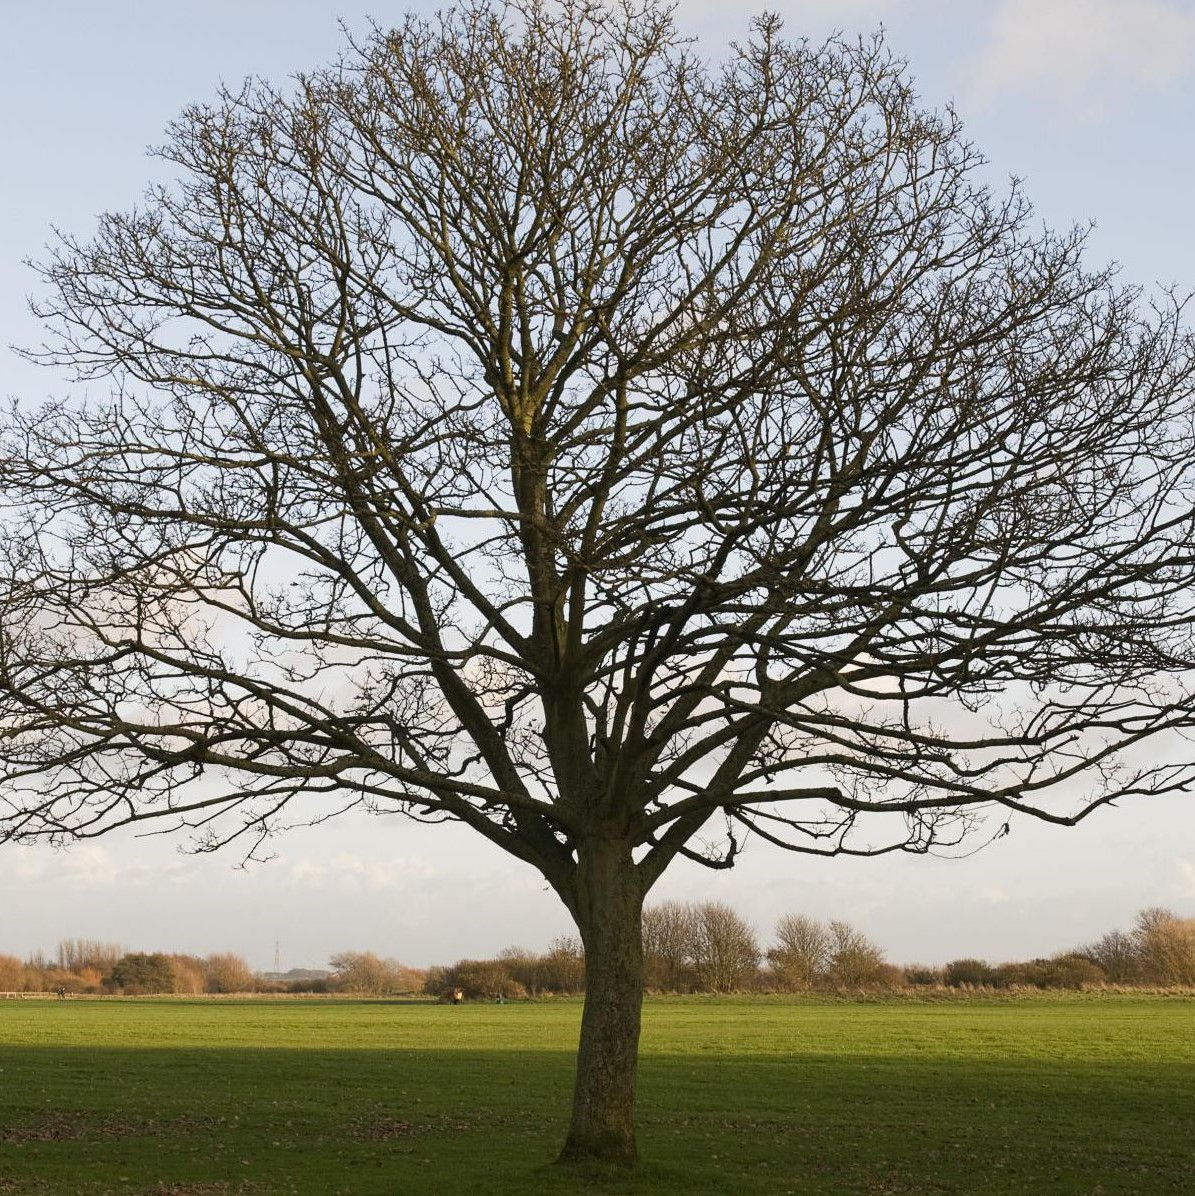
\includegraphics[width=\textwidth]{img/nat_pat_04.jpg}
		\caption{}  
	\end{subfigure}
	\caption{}
	\label{fig:nat_pet}
\end{figure*}

Mint ahogy azt Kovács Nemere is kifejti a A képzőművészet története III. részében az ősművészeteknél \cite{nemerekepzHomHuveszet} a természeti motívumok és eszközök már az ősidők óta részét képezik az emberi művészetnek. Amikor a barlangrajzokat készítették számukra az elsődleges forrás a természet volt, (\ref{fig:osi}. ábra).
Abban az időben az ember csak a környezetében található tárgyakat tudta felhasználni és az akkor kialakuló emberi kreativitás által az egyszerű eszközök és alapanyagokból létrehozni a művészetet. A saját tapasztalatuk útján jöttek rá, hogy miként tudják felhasználni az őket körülvevő anyagokat: növények, ásványok, rovarok és mindent amit megismert az elméjük. Az így megismert és létrehozott alapanyagokkal kezdték újrateremteni az érzékelt világot primitív művészeti formákban, például barlang rajzok, kezdetleges bőr művek vagy éppen primitív szövetek formályában. A legleső szín, ami az ősi művészetekben megjelent a sárga és annak árnyalatai voltak, amit különböző növényekből tudtak elő állítani.
A nomád, vándorló népek napjainkig őrzik ez az erős természettel való együttélést. Színezékeik mind az őket körülvevő és épp aktuálisan megtalálható növényből készülnek.

\begin{figure}[h!]
	\centering
	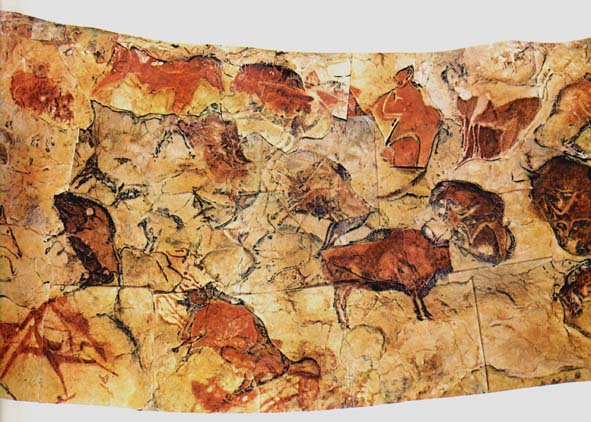
\includegraphics[width=0.5\textwidth]{img/osi.jpg}
	\caption{Barlang rajz}
	\label{fig:osi}
\end{figure}

Első ránézésre a természet néha egy kaotikus képet mutat magáról, amit nehéz értelmezni, de az idő haladtával az ember elkezdete ezeket a kaotikus mintázattokat vizsgálni és értelmezni és rájöttek, hogy ebben a kaotikus képben valamelyest rejlik egy matematikai rend.

A természetben megfigyelhető minták, alakzatok, formák rendszeresek ismétlődők ilyen mintázatok a fraktálok (\ref{fig:fraktal}. ábra). A fraktálok egyik legismertebb tulajdonsága, mint ahogy azt Mandelbrot Benoit B. is kifejti \cite{mandelbrot1982fractal} önhasonlóság, a természetben nagyon sok helyen találkozhatunk ilyen mintázattal, nem csak formai, hanem rendszer szinten is nagyon jó példák erre a fák ők is természetes fraktálok abban az értelemben is, hogy sokszorosítják magukat és, hogy az erdő és természet létrehozza a biológiai önhasonlóságot. 

\begin{figure}[h!]
	\centering
	\begin{subfigure}[b]{0.4\linewidth}
	  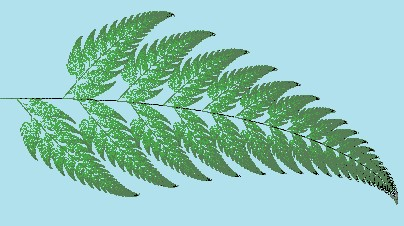
\includegraphics[width=\linewidth]{img/fraktal_01.jpg}
	  \caption{}
	\end{subfigure}
	\begin{subfigure}[b]{0.47\linewidth}
	  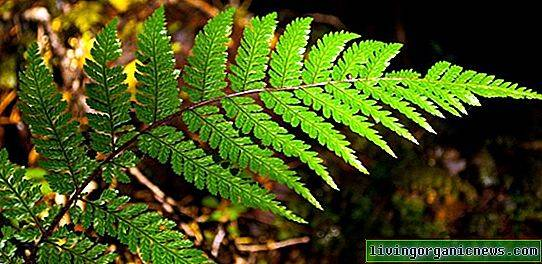
\includegraphics[width=\linewidth]{img/fraktal_02.jpg}
	  \caption{}
	\end{subfigure}
	\caption{Fraktálok és páfrány levél}
	\label{fig:fraktal}
  \end{figure}

A természetben persze nem csak ilyen mintázatok jelennek meg, hanem egyszerűbb struktúrák is, mint például a foltok, a csíkok, a spirálok, a fodrok, az elágazás vagy a repedések, törések és a növények növekedése során lerajzolt formák is ebbe a körbe tartoznak.

Dolgozatom célja hogy megmutassam miként jelennek meg a művészeti alkotásokban a természeti minták és motívumok, mint szerkezeti és strukturális szinten. Ezt egy technikán keresztül mutatom be, amelynek alapja a természetes alapanyagok, nevezetesen az indigó és a természeti motívumokból inspirálódik. 

\section{Alapfogalmak}
A dolgozatírás közben felhasznált alapvető és szükséges fogalmak:
\begin{itemize}
	\item \textbf{Motívum} \\  A művészetekben a legkisebb önálló kifejezőegység, amely a mű során általában ismétlődik. A folklór - népművészet alkotás legkisebb tartalmi egysége, amely átvétel után is felismerhető marad.
	\item \textbf{Organikus} \\ szerves, növényi , állati eredetű alkotóelem, 
	\item \textbf{Ornamentika} \\ (a lat. orno, 'felszerel, díszít' szóból): egy-egy kor, nép, műfaj vagy stílus díszítményeinek összessége. - Lehet mértani, növényi, figurális v. vegyes összetételű.
	\item \textbf{Festék} \\ Tágabb, köznapi értelemben mindenféle anyag, ami egy tárgy színét megváltoztatja: fedőfesték, máz, zománc, lakk, pasztell, lazúr stb. Szűkebb értelemben: a felületre felvitt, az alapot (szinte) teljesen elfedő, vékony, pigmentált réteg. A kötőanyagtól függően lehet: enyv-, olaj-, akril*-, tempera**-, viasz-, méz-, gyanta- stb. festék.
	\item \textbf{Színezék} \\
	Vízben oldható színezőanyag, mely kötőanyagot nem tartalmaz, jellemzően a kelmefestés kelléke. Az anyagot nem fedi el a színezék, hanem beleivódik a rostjaiba, a pigment kémiailag kötődik az anyaghoz. A létrejövő szín és teltsége függ a textilanyag fehérségétől, a kezelés időtartamától, a festőoldat sűrűségétől, az elő- és utókezelés módjától, anyagától (pácoktól*), ezek vegyi összetételétől, olykor más tényezőktől is.
	\item \textbf{Kelmefestés / Kékfestés} \\ 
	Egy textíliákon alkalmazott színmintázási technológia, amely nevét onnan kapta, hogy a minta eredeti formájában jellegzetesen kék alapon fehér színben jelenik meg.
	\end{itemize}

\section{A természet mint, inspirációs forrás}
A művészi kifejezőeszközök mentén az alkotó megfigyeli a természetet és gyakran lemásolja azt, mindeközben egy absztrakciós folyamat alá veti, mindeközben egyszerűsödik a természeti motívum, újra értelmeződig és adaptálódik megfelelő médiumra.
%A művészet utánozhatja a természetet azáltal, hogy egy absztrakción keresztül újra értelmezi azt, vagy képes teljesen lemásolni.

%A művészet kinyit olyan ajtókat nekünk a természet felé ami a természet  bonyolultságára és szépségére hívja fel figyelmünket, amit semmi képen nem lehet elszalasztani.

Lehet egy egyszerű művészeti kép, ami segít értelmezi a természetet vagy lehet egy kihívást jelentő darab ami kifejezi a emberi kapcsolatot a természettel.\cite{art_nature} 
A természet megfigyelése mentén végbemenő gondolkodásmód által való művészeti lehetőségeket  add nekünk egy olyan látásmód kialakítására ami maga a természetben előforduló anyagokkal, tárgyakkal való munkát helyezi a művészeti folyamat közép pontjába, mint például levelek, botok, ágak, termések, víz, kövek és ezekhez hasonló természeti tárgyak használata.
Mindezek megfigyelése és azok tulajdonságainak értelmezése a design gondolkodásban is jelen van. Ezt nevezzük Anyag vezérelt tervezői gondolkodásnak vagy Material Driven Design-nak \cite{karana2015material}.
Kreatív módon való felhasználást késztetést érzünk új művészeti tárgyak készítésére.
\cite{meller2002textile}
Ez a fajta művészeti filozófia fenntartja a kapcsolatot az őskori emberekkel és a természettel. Transzcendentálissá és az időn átívelővé téve természetet, ember és művészetet.

Manapság sok kortás művész messze van attól a folyamtól, hogy ténylegesen saját maga hozzon létre bármilyen alapanyagot, mint például festék vagy pigmentek a saját munkájának a megvalósításában. Ezzel ellentétben egyre kevesebb olyan művész és mesterember található aki a teljes alkotói folyamatot átlátja és végig vezeti.

\vspace{2 mm}
Egy közismert mai kortás alkotó, aki művészetében visszanyúl az ősi alapanyagokhoz Andy Goldsworthy. Olyan természetes anyagokat használt fel munkái során, mint például levelek, kövek és hely- specifikus szobrokat készített amelyek tükrözik az anyagok és a természet közöti ősi kapcsolatot.Munkáinak az elkészítési ideje hosszú folyamat, a felhasznált  alapanyagok össze gyűjtése és előkészítése mélyíti el azt az ősi kapcsolatot ami művész és műalkotás között ki tudd alakulni.
A kész művei fényképformájában maradtak fent mivel ezek az alkotások a természetben helyezkednek el és semmilyen olyan alkotó elemet nem tartalmaztak, ami megóvná a természet viszontagságaitól és lassan elamortizálódtak ilyen módon fejezte ki, hogy a tényleges műalkotás múlandó.

\vspace{2 mm}
Hannah Jones a Nike fenntarthatóság \cite{nike} létre hozója,célja az volt hogy a fenntarthatósági kihívásokat végig vigye. 
Számára a forma és a funkció több mint egy desing elem, ezek a társadalmi és környezeti forradalmi alapok közzé tartoznak ezzel megzavarva környezetében lévő embereket, és a világot újra gondolják az anyagok használatát .
A fenntarthatóság megköveteli a rendszer megváltoztatását kivül belül.

\vspace{2 mm}
Egy ilyen kortás ritkaság a hagyományos japán kerámia a Tamba Yaki \cite{tambayaki}, ez az egyik a 6 hagyományos fazekas stílusnak japánban, több mint 800 éves múltra tekint vissza. Egyik jellegzetessége a régió Kiotó és Oszaka között a Kurakura és a Wadajaki hegyek között elhelyezkedő hegyi falvak és az ott található alapanyagok. Ma is a mesterek maguk gyűjtik és készítik el a kerámiákhoz használt agyagot és mázat, amit a mesterek saját titkos receptúrája alapján, de a legfontosabb, hogy csak is a régióból származó természetes összetevőkből állít elő. A kerámiák felületén kialakított minták és motívumok is a természetből származnak, amit lenyomatolással levelek termések felhasználásával vagy festés - karcolás váltogatásával állítanak elő. Ez az irányzat az egyszerű és letisztult természetes vonal vezetéséről ismert, és hogy mindennapi használati tárgyakat állítanak elő. Az, hogy az ősi technikák formák és minták túlélték  a századokat és még ma is több műhely és mester dolgozik annak köszönhető, hogy mindig is lehetőséget biztosítottak a különböző művészeti határsoknak formavilágoknak a beemelésére és a 20. század elején megjelenő Japán Kézműves mozgalomnak.



% \section{A természet a magyar kortás művészetben}

% Ide bármilyen kortárs magyar művészt aki valamilyen természet közelit csinál.

% \subsection{Színanyagok}
% A természetben előforduló pigment anyagok melyek felhasználásra kerülnek a legkülönfélébb művészeti alkotásokban:
% Indigó, Bíbor, 
% \subsection{Eszközök}
% Nyomódúc. textilminták előállítására használt fa mintanyomó eszköz, leginkább puha és keményebb fa fajtákból készült mint például gesztenye fa vagy dió fa vagy tölgy vagy bükk
% \section{A természet a saját mintáimban}
% Az eddig munkáim során a ösztönösen a természetnél lyukadtam ki, de miért pont a természetnél azt még az elején magam se tudtam, ahogy elkezdtem a különböző feladataim során a tanulmányokat mindig a fák és terméseik lettek a fókuszban e fafajták közül hármat választottam.

% Próbáltam olyan természeti elemeket keresni, amik a minden napi köztudatban benne vannak és ezeket a természeti formákat mindenki ismeri és találkozótt vele és már felhasználta ezeket valamiyen formában. 

% Ezek a termések a dió, a makk és a gesztenye volt \ref{fig:sajat1}. ábra.
% Ezeket a terméseket szeretném egy újabb, modernebb irányban vinni ahol ezek a természeti elemek más arculatban, könnyed vonal rendszerrel, de mégis felismerhető minta ként jelenjenke meg az emberek számára.

% \begin{figure}[h!]
% 	\centering
% 	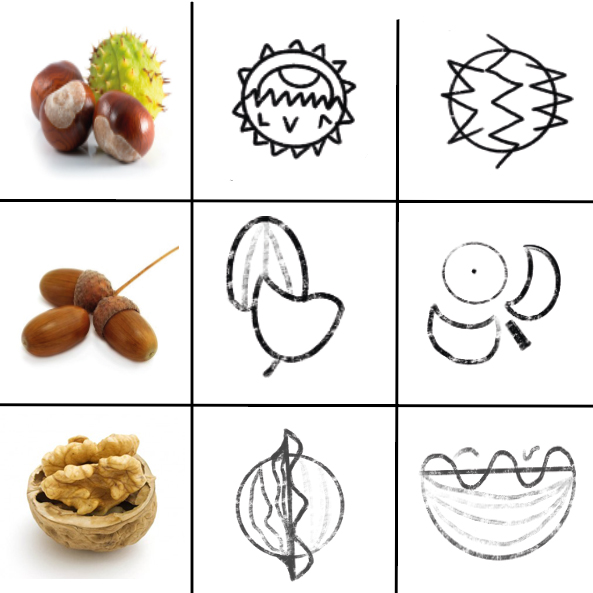
\includegraphics[width=0.8\textwidth]{img/sajat01.jpg}
% 	\caption{Saját mintakészlet fejlődés. Gesztenye - Mak - Dió}
% 	\label{fig:sajat1}
% \end{figure}